\documentclass[12pt]{article}
\usepackage{fancyhdr}
\usepackage{color}
\usepackage{multicol}
\usepackage{enumitem}
\usepackage{graphicx}
\usepackage{sectsty}
\usepackage{amsmath}
\usepackage{amssymb}
\usepackage{hyperref}
\usepackage{array}
\newcommand{\sectionbreak}{\clearpage}
\usepackage{lscape}

\usepackage{tikz}
	\usetikzlibrary{arrows,shapes,trees}

\usepackage{tkz-euclide}
\usetkzobj{all}

\allsectionsfont{\centering}

\usepackage{draftwatermark}
	\SetWatermarkText{wolf-math.com}
	\SetWatermarkScale{5}
	\SetWatermarkAngle{90}
	\SetWatermarkLightness{1}

\usepackage[margin=.75in, headsep=0pt]{geometry}
\setlength{\parindent}{0cm}
\pagestyle{empty}


\begin{document}

\section{Graphing Trigonometric Functions}

\subsection{Goals}

\textbf{I will be able to} graph a trigonometric functions using a unit circle as a guide.\\

\textbf{I will be able to} translate and transform trigonometric funtions.\\

\subsection{Standards}

\subsection{Connections}

\clearpage

\section*{Graphing a Sine Wave}

Recall that the radius of the unit circle is 1, and the points on the unit circle $(x,y)$ also correspond to the trig functions $(\cos, \sin)$. \\

We can now draw a graph where the $x$ axis is the \emph{angle} and the $y$ axis is the \emph{trig function}: $f(x)=\sin(x)$.\\

\section*{Graphing a Cosine Wave}

Now draw a graph where the $x$ axis is the \emph{angle} and the $y$ axis is the \emph{trig function}: $f(x)=\cos(x)$.\\


\begin{landscape}

\section*{Graphing a Sine Wave}

Recall that the radius of the unit circle is 1, and the points on the unit circle $(x,y)$ also correspond to the trig functions $(\cos, \sin)$. \\

We can now draw a graph where the $x$ axis is the \emph{angle} and the $y$ axis is the \emph{trig function}: $f(x)=\sin(x)$.\\

\vspace{1in}

\begin{tiny}
    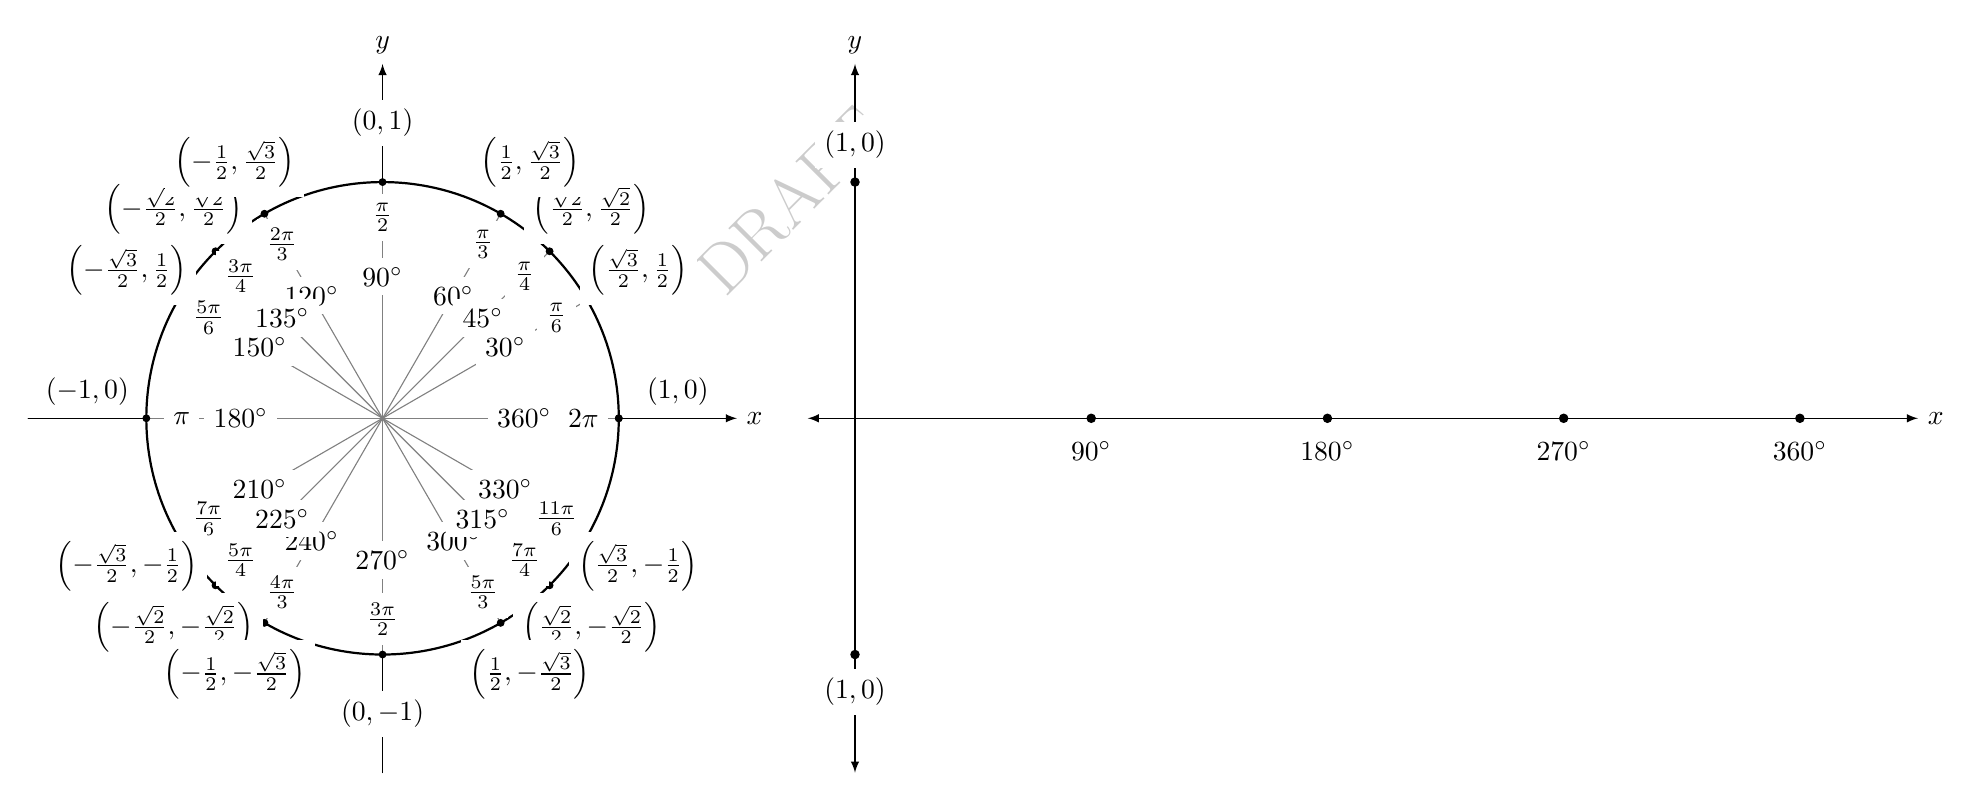
\begin{tikzpicture}[scale=3,cap=round,>=latex]
        % draw the coordinates
        \draw[->] (-1.5cm,0cm) -- (1.5cm,0cm) node[right,fill=white] {$x$};
        \draw[->] (0cm,-1.5cm) -- (0cm,1.5cm) node[above,fill=white] {$y$};

        % draw the unit circle
        \draw[thick] (0cm,0cm) circle(1cm);

        \foreach \x in {0,30,...,360} {
                % lines from center to point
                \draw[gray] (0cm,0cm) -- (\x:1cm);
                % dots at each point
                \filldraw[black] (\x:1cm) circle(0.4pt);
                % draw each angle in degrees
                \draw (\x:0.6cm) node[fill=white] {$\x^\circ$};
        }

		\foreach \x in {45,135,225,315}{
				\draw[gray](0cm,0cm) -- (\x:1cm);
				\filldraw[black] (\x:1cm) circle(0.4pt);
				\draw (\x:0.6cm) node[fill=white] {$\x^\circ$};
		}

        % draw each angle in radians
        \foreach \x/\xtext in {
            30/\frac{\pi}{6},
            45/\frac{\pi}{4},
            60/\frac{\pi}{3},
            90/\frac{\pi}{2},
            120/\frac{2\pi}{3},
            135/\frac{3\pi}{4},
            150/\frac{5\pi}{6},
            180/\pi,
            210/\frac{7\pi}{6},
            225/\frac{5\pi}{4},
            240/\frac{4\pi}{3},
            270/\frac{3\pi}{2},
            300/\frac{5\pi}{3},
            315/\frac{7\pi}{4},
            330/\frac{11\pi}{6},
            360/2\pi}
                \draw (\x:0.85cm) node[fill=white] {$\xtext$};

        \foreach \x/\xtext/\y in {
            % the coordinates for the first quadrant
            30/\frac{\sqrt{3}}{2}/\frac{1}{2},
            45/\frac{\sqrt{2}}{2}/\frac{\sqrt{2}}{2},
            60/\frac{1}{2}/\frac{\sqrt{3}}{2},
            % the coordinates for the second quadrant
            150/-\frac{\sqrt{3}}{2}/\frac{1}{2},
            135/-\frac{\sqrt{2}}{2}/\frac{\sqrt{2}}{2},
            120/-\frac{1}{2}/\frac{\sqrt{3}}{2},
            % the coordinates for the third quadrant
            210/-\frac{\sqrt{3}}{2}/-\frac{1}{2},
            225/-\frac{\sqrt{2}}{2}/-\frac{\sqrt{2}}{2},
            240/-\frac{1}{2}/-\frac{\sqrt{3}}{2},
            % the coordinates for the fourth quadrant
            330/\frac{\sqrt{3}}{2}/-\frac{1}{2},
            315/\frac{\sqrt{2}}{2}/-\frac{\sqrt{2}}{2},
            300/\frac{1}{2}/-\frac{\sqrt{3}}{2}}
                \draw (\x:1.25cm) node[fill=white] {$\left(\xtext,\y\right)$};

        % draw the horizontal and vertical coordinates
        % the placement is better this way
        \draw (-1.25cm,0cm) node[above=1pt] {$(-1,0)$}
              (1.25cm,0cm)  node[above=1pt] {$(1,0)$}
              (0cm,-1.25cm) node[fill=white] {$(0,-1)$}
              (0cm,1.25cm)  node[fill=white] {$(0,1)$};

        % draw the coordinates
        \draw[<->] (1.8cm,0cm) -- (6.5cm,0cm) node[right,fill=white] {$x$};
        \draw[<->] (2cm,-1.5cm) -- (2cm,1.5cm) node[above,fill=white] {$y$};
        
        \draw [fill=black] (2cm,1cm) circle (.5pt);
        \draw (2cm,1cm) node[above=5pt, fill=white] {$(1,0)$};
        
        \draw [fill=black] (2cm,-1cm) circle (.5pt);
        \draw (2cm,-1cm) node[below=5pt, fill=white] {$(1,0)$};
        
        \draw [fill=black] (3cm,0cm) circle (.5pt);
        \draw (3cm,0cm) node[below=5pt, fill=white] {$90^\circ$};
        
        \draw [fill=black] (4cm,0cm) circle (.5pt);
        \draw (4cm,0cm) node[below=5pt, fill=white] {$180^\circ$};
        
        \draw [fill=black] (5cm,0cm) circle (.5pt);
        \draw (5cm,0cm) node[below=5pt, fill=white] {$270^\circ$};
        
        \draw [fill=black] (6cm,0cm) circle (.5pt);
        \draw (6cm,0cm) node[below=5pt, fill=white] {$360^\circ$};
\end{tikzpicture}
\end{tiny}

\clearpage

\section*{Graphing a Cosine Wave}

Now draw a graph where the $x$ axis is the \emph{angle} and the $y$ axis is the \emph{trig function}: $f(x)=\cos(x)$.\\

\vspace{1in}

\begin{tiny}
    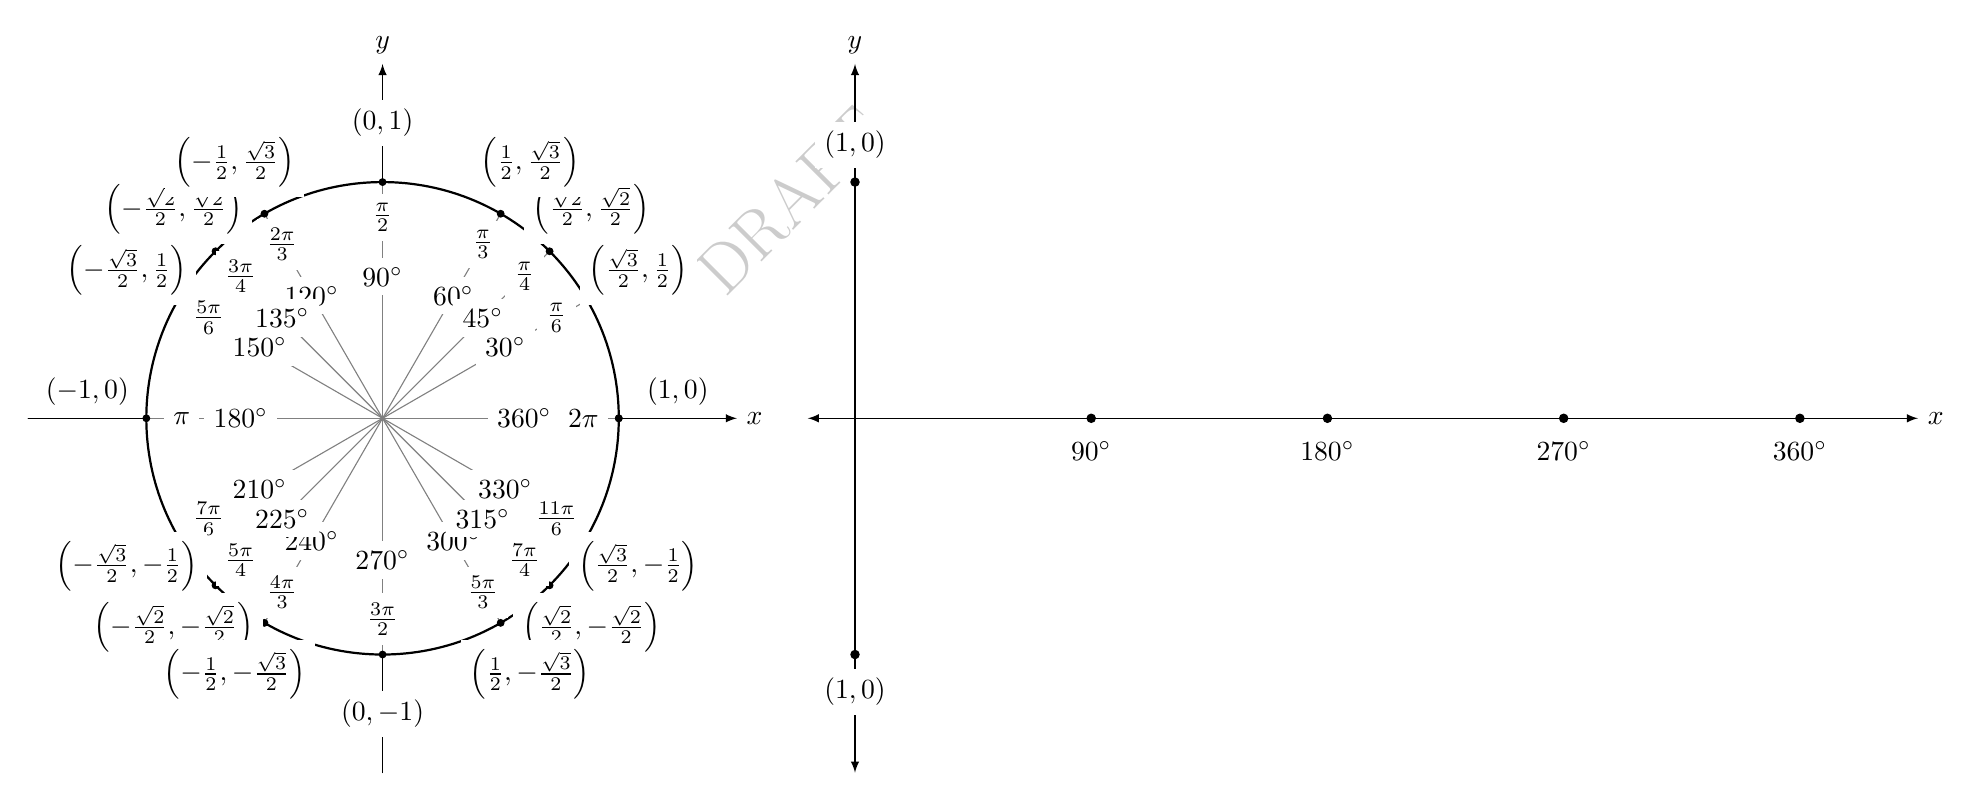
\begin{tikzpicture}[scale=3,cap=round,>=latex]
        % draw the coordinates
        \draw[->] (-1.5cm,0cm) -- (1.5cm,0cm) node[right,fill=white] {$x$};
        \draw[->] (0cm,-1.5cm) -- (0cm,1.5cm) node[above,fill=white] {$y$};

        % draw the unit circle
        \draw[thick] (0cm,0cm) circle(1cm);

        \foreach \x in {0,30,...,360} {
                % lines from center to point
                \draw[gray] (0cm,0cm) -- (\x:1cm);
                % dots at each point
                \filldraw[black] (\x:1cm) circle(0.4pt);
                % draw each angle in degrees
                \draw (\x:0.6cm) node[fill=white] {$\x^\circ$};
        }

		\foreach \x in {45,135,225,315}{
				\draw[gray](0cm,0cm) -- (\x:1cm);
				\filldraw[black] (\x:1cm) circle(0.4pt);
				\draw (\x:0.6cm) node[fill=white] {$\x^\circ$};
		}

        % draw each angle in radians
        \foreach \x/\xtext in {
            30/\frac{\pi}{6},
            45/\frac{\pi}{4},
            60/\frac{\pi}{3},
            90/\frac{\pi}{2},
            120/\frac{2\pi}{3},
            135/\frac{3\pi}{4},
            150/\frac{5\pi}{6},
            180/\pi,
            210/\frac{7\pi}{6},
            225/\frac{5\pi}{4},
            240/\frac{4\pi}{3},
            270/\frac{3\pi}{2},
            300/\frac{5\pi}{3},
            315/\frac{7\pi}{4},
            330/\frac{11\pi}{6},
            360/2\pi}
                \draw (\x:0.85cm) node[fill=white] {$\xtext$};

        \foreach \x/\xtext/\y in {
            % the coordinates for the first quadrant
            30/\frac{\sqrt{3}}{2}/\frac{1}{2},
            45/\frac{\sqrt{2}}{2}/\frac{\sqrt{2}}{2},
            60/\frac{1}{2}/\frac{\sqrt{3}}{2},
            % the coordinates for the second quadrant
            150/-\frac{\sqrt{3}}{2}/\frac{1}{2},
            135/-\frac{\sqrt{2}}{2}/\frac{\sqrt{2}}{2},
            120/-\frac{1}{2}/\frac{\sqrt{3}}{2},
            % the coordinates for the third quadrant
            210/-\frac{\sqrt{3}}{2}/-\frac{1}{2},
            225/-\frac{\sqrt{2}}{2}/-\frac{\sqrt{2}}{2},
            240/-\frac{1}{2}/-\frac{\sqrt{3}}{2},
            % the coordinates for the fourth quadrant
            330/\frac{\sqrt{3}}{2}/-\frac{1}{2},
            315/\frac{\sqrt{2}}{2}/-\frac{\sqrt{2}}{2},
            300/\frac{1}{2}/-\frac{\sqrt{3}}{2}}
                \draw (\x:1.25cm) node[fill=white] {$\left(\xtext,\y\right)$};

        % draw the horizontal and vertical coordinates
        % the placement is better this way
        \draw (-1.25cm,0cm) node[above=1pt] {$(-1,0)$}
              (1.25cm,0cm)  node[above=1pt] {$(1,0)$}
              (0cm,-1.25cm) node[fill=white] {$(0,-1)$}
              (0cm,1.25cm)  node[fill=white] {$(0,1)$};

        % draw the coordinates
        \draw[<->] (1.8cm,0cm) -- (6.5cm,0cm) node[right,fill=white] {$x$};
        \draw[<->] (2cm,-1.5cm) -- (2cm,1.5cm) node[above,fill=white] {$y$};
        
        \draw [fill=black] (2cm,1cm) circle (.5pt);
        \draw (2cm,1cm) node[above=5pt, fill=white] {$(1,0)$};
        
        \draw [fill=black] (2cm,-1cm) circle (.5pt);
        \draw (2cm,-1cm) node[below=5pt, fill=white] {$(1,0)$};
        
        \draw [fill=black] (3cm,0cm) circle (.5pt);
        \draw (3cm,0cm) node[below=5pt, fill=white] {$90^\circ$};
        
        \draw [fill=black] (4cm,0cm) circle (.5pt);
        \draw (4cm,0cm) node[below=5pt, fill=white] {$180^\circ$};
        
        \draw [fill=black] (5cm,0cm) circle (.5pt);
        \draw (5cm,0cm) node[below=5pt, fill=white] {$270^\circ$};
        
        \draw [fill=black] (6cm,0cm) circle (.5pt);
        \draw (6cm,0cm) node[below=5pt, fill=white] {$360^\circ$};
\end{tikzpicture}
\end{tiny}

\clearpage

\section*{Multipliers}

What happens if we multiply something in front of the wave?\\

$$f(x)=2\cdot \sin(x)$$

\begin{tiny}
    \begin{tikzpicture}[scale=3,cap=round,>=latex]

        \draw[<->] (1.8cm,0cm) -- (6.5cm,0cm) node[right,fill=white] {$x$};
        \draw[<->] (2cm,-1.5cm) -- (2cm,1.5cm) node[above,fill=white] {$y$};
        
        \draw [fill=black] (2cm,1cm) circle (.5pt);
        \draw (2cm,1cm) node[above=5pt, fill=white] {$(1,0)$};
        
        \draw [fill=black] (2cm,-1cm) circle (.5pt);
        \draw (2cm,-1cm) node[below=5pt, fill=white] {$(1,0)$};
        
        \draw [fill=black] (3cm,0cm) circle (.5pt);
        \draw (3cm,0cm) node[below=5pt, fill=white] {$90^\circ$};
        
        \draw [fill=black] (4cm,0cm) circle (.5pt);
        \draw (4cm,0cm) node[below=5pt, fill=white] {$180^\circ$};
        
        \draw [fill=black] (5cm,0cm) circle (.5pt);
        \draw (5cm,0cm) node[below=5pt, fill=white] {$270^\circ$};
        
        \draw [fill=black] (6cm,0cm) circle (.5pt);
        \draw (6cm,0cm) node[below=5pt, fill=white] {$360^\circ$};
\end{tikzpicture}
\end{tiny}

\end{landscape}

\end{document}
